\documentclass[a4paper,oneside,article,danish,table]{memoir}
\checkandfixthelayout
\XeTeXtracingfonts= 1
\usepackage{babel,microtype,verbatim,threeparttable,amsmath,amssymb,unicode-math,hyperref,siunitx,mhchem,tikz,pgfplots,tikz-timing}
\sisetup{per-mode=symbol}
\microtypesetup{final,verbose=silent}
\usetikzlibrary{mindmap,arrows,positioning,shapes}
\setmainfont[Ligatures={TeX}]{Arno Pro}
%\setmainfont{Linux Libertine O}
\setmathfont{[Asana-Math]}
%\hfuzz=1pt
\usepackage[margin,draft]{fixme}
\fxusetheme{color}

\newcommand{\authorvar}{Mathias~Dannesbo}
\newcommand{\pretitlevar}{Programmering C eksamen:}
\newcommand{\titlevar}{Swagway Debugger} 
\newcommand{\subtitlevar}{0} 
\newcommand{\datevar}{\today} 
\newcommand{\subjectvar}{Programmering C}
\newcommand{\classvar}{}
\newcommand{\teachervar}{}

\makepagestyle{articlehead}
\makeevenhead{articlehead}{}{\titlevar}{}
\makeevenfoot{articlehead}{}{\thepage}{}
\makeoddhead{articlehead}{}{\titlevar}{}
\makeoddfoot{articlehead}{}{}{\thepage}
\pagestyle{articlehead}

\usepackage{listings,textcomp}
\lstset{language=[Sharp]C,
%  morekeywords={[2]abs,acos,asin,atan,atan2,ceil,constrain,cos,degrees,exp,floor,log,map,max,min,radians,random,randomSeed,round,sin,sq,sqrt,tan,bitRead,bitWrite,bitSet,bitClear,bit,highByte,lowByte,analogReference,analogRead,analogWrite,attachInterrupt,detachInterrupt,delay,delayMicroseconds,digitalWrite,digitalRead,interrupts,millis,micros,noInterrupts,noTone,pinMode,pulseIn,shiftIn,shiftOut,tone,Serial,Serial1,Serial2,Serial3,begin,end,peek,read,print,println,available,flush,setTimeout,find,findUntil,parseInt,parseFloat,readBytes,readBytesUntil},
  keywordstyle={\bfseries\color[rgb]{0,0,1}},
%  keywordstyle={[2]\bfseries\color[rgb]{0.8,0.33,0}},
  identifierstyle=\ttfamily,
  commentstyle=\color[rgb]{0.133,0.545,0.133},
  stringstyle=\color[rgb]{0.627,0.126,0.941},
  showstringspaces=false,
  basicstyle=\small\ttfamily,
  numberstyle=\footnotesize,
  numbers=left,
  stepnumber=1,
  numbersep=10pt,
  tabsize=2,
  breaklines=true,
  breakatwhitespace=false,
  upquote=true,
  extendedchars=true,
  literate={æ}{{\ae}}1
    {ø}{{\o}}1
    {å}{{\aa}}1
}

\newcommand{\form}[2]{\lstinputlisting[firstnumber=#1,firstline=#1,lastline=#2]{../Software/Form1.cs}}
\newcommand{\boarddate}[1]{\textcolor{blue!80!black}{#1}}
\newcommand{\issue}[1]{\textsuperscript{\textcolor{blue!80!black}{\href{https://github.com/neic/Swagway/issues/#1}{\##1}}}}


\begin{document}
% \includepdf{forside.pdf} \clearpage%------------------------ Forside

\begin{center}
  \if\pretitlevar 0
  \else{\Large\pretitlevar\\} \fi
  \textsc{\HUGE\titlevar\\}
  \if\subtitlevar 0
  \else {\Large\subtitlevar\\} \fi
  %\vspace{1em}
  {\LARGE 
  af\\
   \authorvar}\\
 \datevar\\
\end{center}
\begin{abstract}
  This journal is a walk-thorugh of the source code of Swagway Debugger, a Windows application for debugging and tuning filters, e.g. Kalman-filters, on balancing robots and Segway clones. It is made as a part of the Swagway project.
\end{abstract}
\thispagestyle{empty}

\chapter{Indledning}
Formålet med opgaven er at lave et stykke software der kan bruges sammen med forfatterens eksamenprojekt i Teknikfag~A:~El. Formålet med teknikfags projektet er at bygge en Segway klon, en motoriseret selvbalancrende tohjulet trasportenhed. Navnet på Segway klonen er Swagway. Under udviklingen af Swagway blev der behov for et stykke software til at teste et filter.\footnote{Websiden for hele projekter findes på \url{https://github.com/neic/Swagway}. Derfra er der adgang til alt kildekode, rapporter og andre skriftlige fremstillinger.}

\subsubsection{Kort beskrivelse af Swagway funktion}
For at Swagway kan holde sig lodret skal den kende vinklen den er fra lodret. Det udregner den ved at læse data fra to sensorer: et accelerometer og et gyroskob.

Et gyroskob kan måle vinkelhastigheder. Det vil sige ændringer i vinklen. Hvis denne vinkelhastighed integreres over tid finder man vinklen gyroskobet har flyttet sig. Problemet med at integrer gyroskobdata er, at pga. måleusikkerheder vil det målte nulpunkt drive væk fra det fysiske nulpunkt.

Et accelerometer kan måle accelerationer. Man kan med hjælp fra tanges og data fra to akser udregne den vinklen accelerometeret står i forhold til jordens tygdekræft. Problemet med dette er at accelerometer måler alle accelerationer, ikke kun jordens tyngdekræft. Når Swagwayen fx accelerer, bremser eller køre over en sten bliver den udregnet vinkel forkert.

For at komme begge problemer til livs bliver begge sensorer brugt og data fra begge to bliver samlet i et såkaldt Kalman-filter. Kalman-filtret kan tilnærmelses ses som et high-pass og low-pass filter. Det taget de hurtige ændringer (high-pass) fra gyroskob-dataene og bruger accelerometer-dataene til at holde det målte og det fysiske nulpunkt over ens.

\subsubsection{Swagway Debugger}
For at teste om Kalman-filtret er implementeret og tunet korrekt er det nødvendig at sammenligne de tre vinkler fra hhv. gyroskobet, accelerometert og kalmanfiltret. En måde at gøre dette på er ved at sende disse data fra elektronikken på Swagwayen til en PC og vise den grafisk. Det er her Swagway~Debugger-softwaren kommer ind i billedet.

Swagway~Debugger modtager data fra en Arduino mikrocontroller på Swagwayen over en seriel-port og skriver dataene på en graf. Som der står i produktbeskrivelsen:
\begin{quotation}
  Opgaven er at lave software der kan modtage data fra en Arduino over en serielport og visualiserer det. Softwaren er til test af filtereringen af data fra et gyroskop og accelerometer. Softwaren viser bl.a. et rullende plot, samt nogle viserinstrumenter.
\end{quotation}

\chapter{Udførelse}
Swagway~Debugger er skrevet på Windows i C\# som en Windows Form Application. Der er ingen eksterne afhængighedder; det bruger kun Microsoft biblioteker: \fxwarning{Er dette biblioteker?}
\form{9}{12}
Der er fem globale variabler:
\form{18}{23}
De tre første er buffere der bliver brugt til midlertidig at gemme modtaget data i, de to sidste er tællere over antallet af pakker.

\section{Indstillinger}
\begin{figure}[htbp]
  \centering
  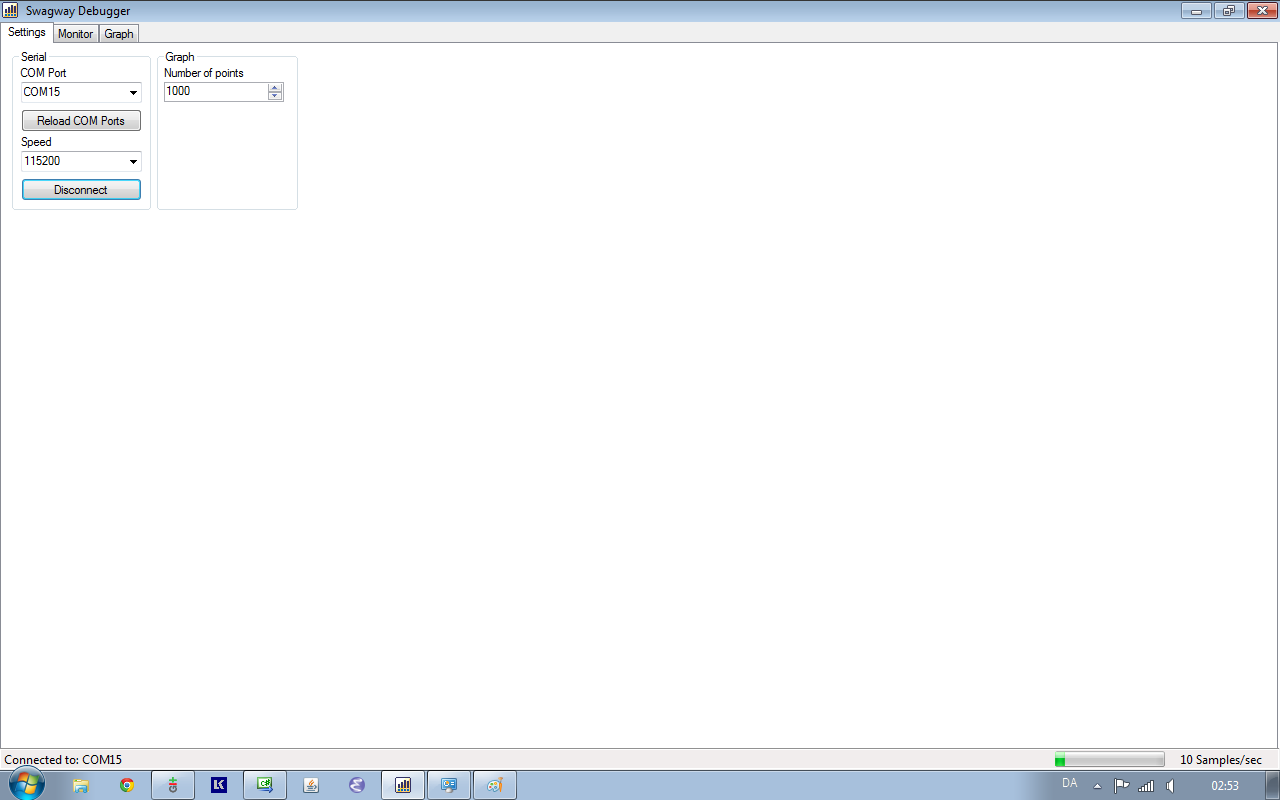
\includegraphics[width=1\textwidth]{settings.png}
  % \caption[]{}
  % \label{fig:}
\end{figure}
Ved opstart af applikationen indlæses alle tilgængelige serial-porte og der sættes en standardinstilling for valget af seriel hastighed:
\form{34}{39}
Ved afslutning af applikationen lukkes en eventuel åben seriel-port:
\form{41}{48}

\texttt{LoadSerialPorts()} kaldes ved opstart og af knappet \texttt{btReload}. Den føjer alle systemets serial-porte til listen, sætter den første seriel-port som standardindstilling og advare i statuslinjen hvis der ikke er fundet seriel-porte:
\form{50}{68}

% btReload_Click undladt
Eventhandleren for \texttt{btConnect} både forbinder og afbryder til en seriel-port. Hvis der er afbrud finder den hvilken serielport og hastighed der er valgt, forbinder og opdaterer statuslinjen og dens egen tekst. Hvis der er oprettet forbindelse afbryder den og ligeledes opdaterer statuslinjen og dens egen tekst:
\form{76}{104}
NumericUpDown-tælleren, \texttt{udPackages}, bestemmer hvor meget data der skal vises på grafen. Når værdien i tælleren ændres ændre den dynamisk skala. Endeligt kalder opdaterer den grafens X-akses maksimal værdi:
\form{106}{125}

\section{Seriel modtagelse og monitor}
\begin{figure}[htbp]
  \centering
  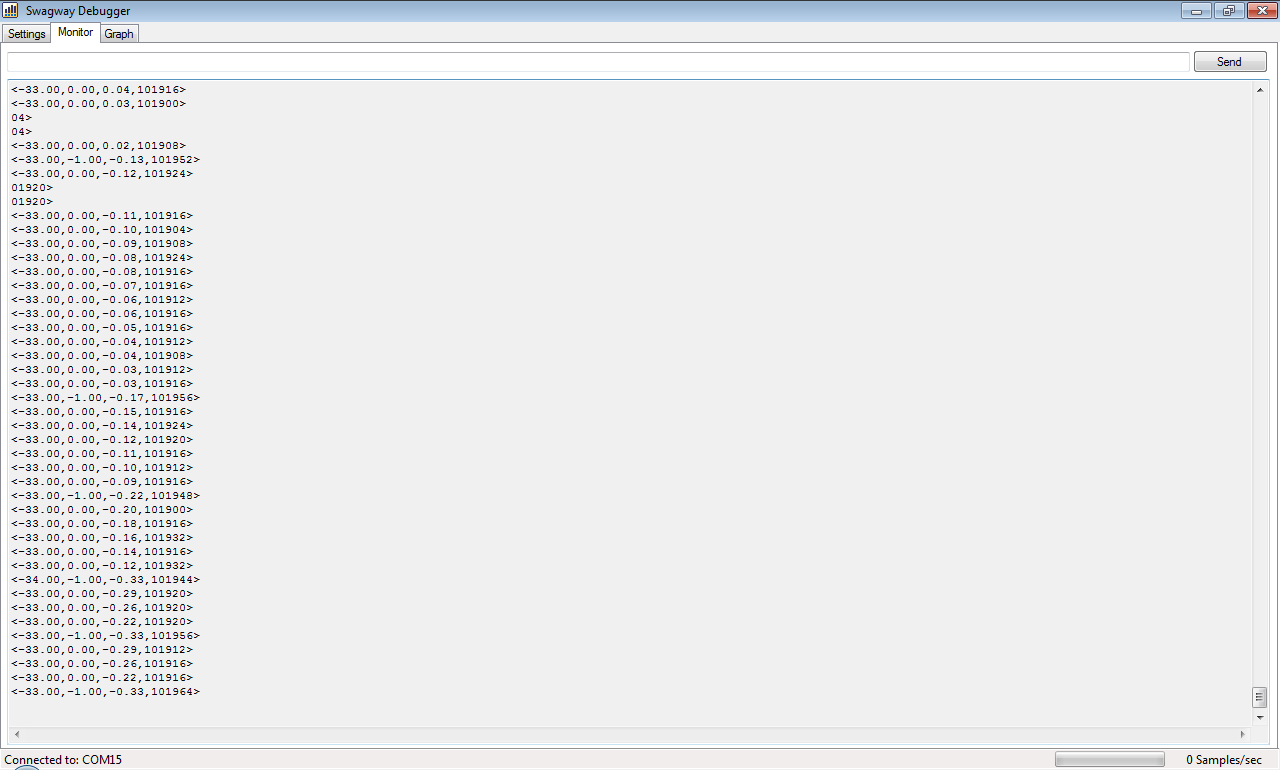
\includegraphics[width=1\textwidth]{monitor.png}
  % \caption[]{}
  % \label{fig:}
\end{figure}
Når der, efter der er forbundet til en seriel-port, ankommer data lægges det i bufferen \texttt{readFromUART} og \texttt{ReadToMonitor} kaldes:
\form{131}{136}
\texttt{ReadToMonitor} Skriver den modtaget data, \texttt{readFromUART}, direkte til monitoren uden at vidrebehandle den. Den undesøger om der er meget data i monitoren og sletter en smugle af det ældste hvis det er tilfældet. Til slut kalder den \texttt{CleanData()}.
\form{138}{149}
Datapakkerne fra Swagwayen er af formen $<\langle \text{gyro} \rangle,\langle \text{acc} \rangle,\langle \text{kalm} \rangle,\langle \text{tid} \rangle>$
\begin{tabbing}
H\=vor\\
\> $\langle \text{gyro} \rangle$ er vinklen målt med gyroskobet med to decimaler og eventuelt negativt fortegn,\\
\> $\langle \text{acc} \rangle$ er vinklen målt med accelerometret med to decimaler og eventuelt negativt fortegn,\\
\> $\langle \text{gyro} \rangle$ er vinklen udregnet af Kalman-filtret  med to decimaler og eventuelt negativt fortegn og\\
\> $\langle \text{tid} \rangle$ er tiden i µS siden sidste pakke blev sendt.
\end{tabbing}
\texttt{CleanData()} tager den rå modtaget data, \texttt{readFromUART}, og tilføjer det til en ny buffer, \texttt{rxStringBuffer}, som allerede indeholder en rest data fra sidste gang. Denne buffer bliver splittet og hver pakke bliver indsat i listen \texttt{rxListBuffer}. Den sidste, ikke fuldstændige, pakke bliver lagt tilbage i \texttt{rxStringBuffer} og er klar til at bliver parret sammen ved næste kald af \texttt{CleanData()}:
\form{151}{157}
Pakkerne i \texttt{rxListBuffer} bliver renset for alt der står efter “>” og bliver undersøgt om de passer ind i formen for en pakke af en regular expression. Hvis den gør dette bliver, pakken splittet til et array af strings for derefter at bliver parset til et array af floats. Dette array bliver givet vidre til til funktionen \texttt{plotPackage()}:
\form{159}{189}

\section{Serial send}
Applikationen kan også sende data. Se hvordan på linje 195--218 af Form1.cs.

\section{Graf}
\begin{figure}[htbp]
  \centering
  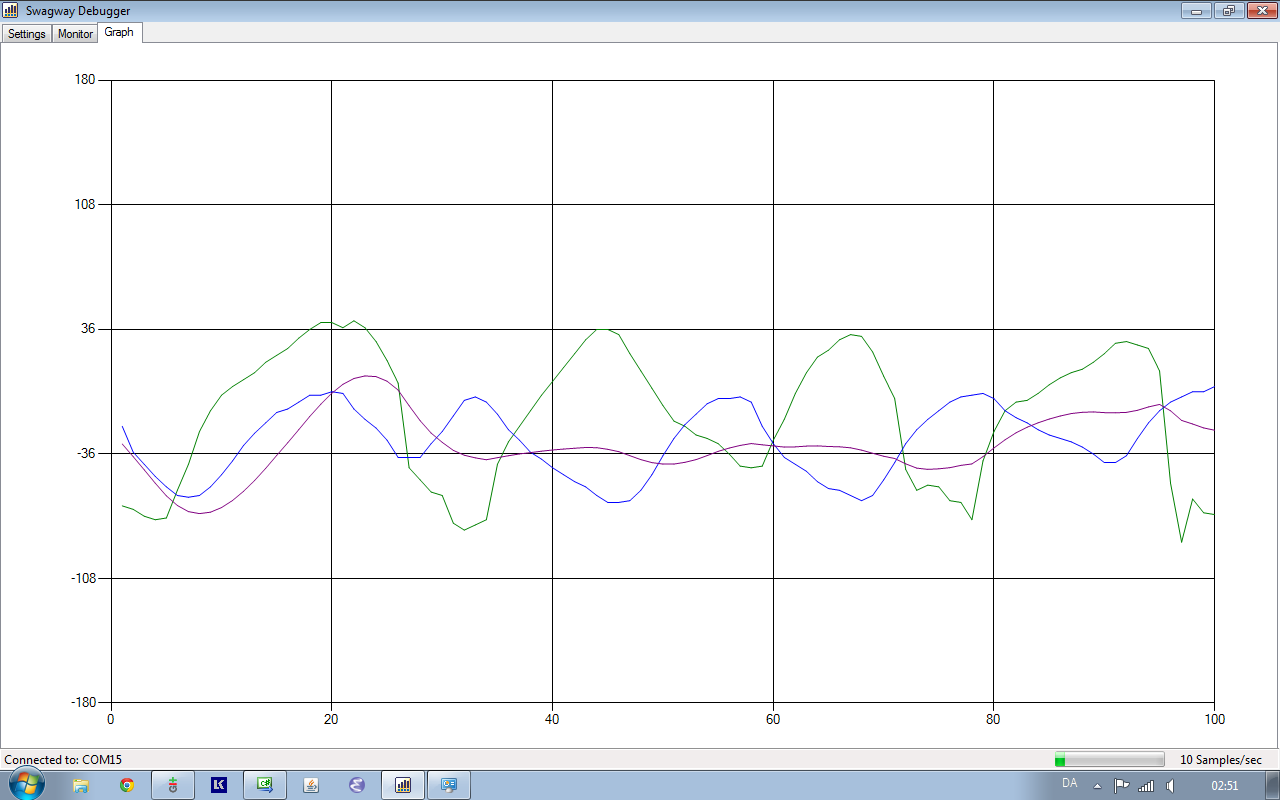
\includegraphics[width=1\textwidth]{graph.png}
  % \caption[]{}
  % \label{fig:}
\end{figure}
Når en ny pakke er blevet renset, bliver hver del af den tilføjet grafen i forskellige serier. Tiden bliver ignoreret. Der bliver så undersøgt om der er pakker over grænseværdien. Hvis der er det bliver de fjernet fra grafen:
\form{224}{239}

\section{Statuslinje}
En timer kalder hvert sekund eventhandleren \texttt{timerSample\_Tick} undersøger hvor mange pakker der er tilføjet det sidste sekund. Den skriver antallet til statuslinjen og opdaterer en statusbjælke:
\form{245}{258}

\chapter{\texttt{Debug\_test.ino}}
Swagway projektet med gyroskob og accelerometer er afleveret, så for at teste Swagway Debugger er der lavet et lille test program til en Arduino. Til Arduinoen er der tilkoblet to potentiometre til at simulere data fra gyroskob og accelerometer. Den del af softwares som har intresse er den som sender pakken med data:
\lstset{language=[Visual]C++,
  morekeywords={[2]abs,acos,asin,atan,atan2,ceil,constrain,cos,degrees,exp,floor,log,map,max,min,radians,random,randomSeed,round,sin,sq,sqrt,tan,bitRead,bitWrite,bitSet,bitClear,bit,highByte,lowByte,analogReference,analogRead,analogWrite,attachInterrupt,detachInterrupt,delay,delayMicroseconds,digitalWrite,digitalRead,interrupts,millis,micros,noInterrupts,noTone,pinMode,pulseIn,shiftIn,shiftOut,tone,Serial,Serial1,Serial2,Serial3,begin,end,peek,read,print,println,available,flush,setTimeout,find,findUntil,parseInt,parseFloat,readBytes,readBytesUntil},
  keywordstyle={[2]\bfseries\color[rgb]{0.8,0.33,0}}}
\lstinputlisting[firstnumber=88,firstline=88,lastline=99]{../Software/Debug_test/Debug_test.ino}

\chapter{Konklusion}
Software blev udviklet og opfyldte både de mål der blev sat samt at hjælpe med Teknologi~A projektet.
\end{document}